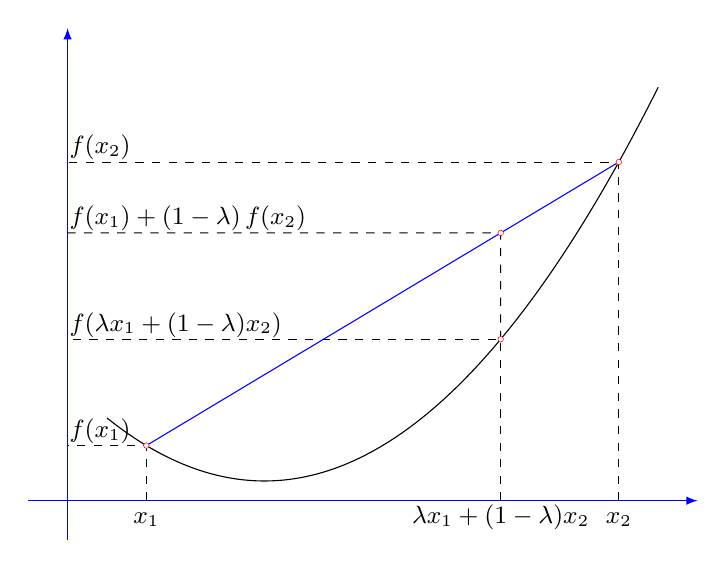
\begin{tikzpicture}[declare function={f(\x)=(\x-1)*(\x-1)/2 +
0.1;},x={(2.5cm,0)},y={(0,2.5cm)},samples=101,font=\small,inner sep=0.5pt]
\draw[blue,-latex] (-0.2,0) -- (3.2,0);
\draw[blue,-latex] (0,-0.2) -- (0,2.4);
\coordinate (O) at (0,0);
\draw plot[domain=0.2:3,variable=\x] ({\x},{f(\x)});
\foreach [count=\Z] \X/\Y in {0.4/{x_1},2.2/{\lambda x_1 +(1-\lambda) x_2},2.8/{x_2}}
{\draw[dashed] (\X,0) coordinate (X\Z) node[below]{$\strut\Y$} -- (\X,{f(\X)}) coordinate (F\Z)
-- (0,{f(\X)}) node[above right]{$f(\Y)$};}
\draw[blue] (F1) -- (F3);
\draw[dashed] (F2) --
(intersection cs:first line={(X2)--(F2)}, second line={(F1)--(F3)})
coordinate (F4) -- (O|-F4) node[above right]{$f(x_1)+(1-\lambda)\,f(x_2)$};
\foreach \X in {1,...,4}
{\draw[very thin,red,fill=white] (F\X) circle(1pt);}
\end{tikzpicture}

%\begin{tikzpicture}
%\begin{axis}[width=5in,axis equal image,
%    axis lines=middle,
%    xmin=0,xmax=8,
%    xlabel=$x$,ylabel=$y$,
%    ymin=-0.25,ymax=4,
%    xtick={\empty},ytick={\empty}, axis on top
%]
%
%% 
%\addplot[thick,domain=0.25:7,blue,name path = A]  {-x/3 + 2.75} coordinate[pos=0.4] (m) ;
%\draw[thick,blue, name path =B] (0.15,4) .. controls (1,1) and (4,0) .. (6,2) node[pos=0.95, color=black, right]  {$f(x)$} coordinate[pos=0.075] (a1)  coordinate[pos=0.95] (a2);
%\path [name intersections={of=A and B, by={a,b}}];

% 
%\draw[densely dashed] (0,0) -| node[pos=0.5, color=black, label=below:$a$] {}(a1);
%\draw[densely dashed] (0,0) -| node[pos=0.5, color=black, label=below:$x_{1}$] {}(a);
%\draw[densely dashed, name path=D] (3,0) -|node[pos=0.5, color=black, label=below:$\lambda x_{1}+ (1-\lambda)x_{2}$] {} node[pos=1, fill,circle,inner sep=1pt] {}(m);
%\draw[densely dashed] (0,0) -|node[pos=0.5, color=black, label=below:$x_{2}$] {}(b);
%\draw[densely dashed] (0,0) -|node[pos=0.5, color=black, label=below:$b$] {}(a2);
%
% 
%\path [name intersections={of=B and D, by={c}}] node[fill,circle,inner sep=1pt] at (c) {}; 

% 
%\node[anchor=south west, text=black] (d) at (0.75,3) {$f[\lambda x_{1}+(1-\lambda)x_{2}]$};
%\node[anchor=south west, text=black] (e) at (5,2.5) {$\lambda f(x_{1})+(1-\lambda)f(x_{2})$};
%\draw[-{Latex[width=4pt,length=6pt]}, densely dashed] (d) -- (c);
%\draw[-{Latex[width=4pt,length=6pt]}, densely dashed] (e) -- (m);
%\end{axis}
%\end{tikzpicture}
